\input{../../headers/tdheaders.tex}

\section{Conception d'un corps support}

Les éléments d'architecture mécano-soudés sont nombreux. Ils peuvent être comme les exemples des figures \ref{img:image1} et \ref{img:image2} constitués de tubes.

\begin{figure}[!h]
 \begin{minipage}{0.45\linewidth}
  \centering\includegraphics[width=1\linewidth]{img/pont.jpg}
  \caption{Décoration de pont}
  \label{img:image1}
\end{minipage}
\hfill
 \begin{minipage}{0.5\linewidth}
  \centering\includegraphics[width=1\linewidth]{img/Beaubourg.jpg}
  \caption{Centre Beaubourg}
  \label{img:image2}
 \end{minipage}
\end{figure}

\begin{figure}[!h]
 \begin{minipage}{0.58\linewidth}
Afin de s'adapter aux structures verticales, il est nécessaire de créer des éléments supports de tubes afin de les fixer.

Un de ces éléments est présenté sur la figure \ref{img:image3}, un autre fait l'objet de cette étude.

Le support sur lequel s'appuie cette étude a été réalisé par mécano-soudage.
\end{minipage}
\hfill
 \begin{minipage}{0.4\linewidth}
  \centering\includegraphics[width=0.6\linewidth]{img/support.jpg}
  \caption{Support de tube}
  \label{img:image3}
 \end{minipage}
\end{figure}

\paragraph{Question 1:} Indiquer les soudures sur ce document ainsi que la symbolique nécessaire à leur compréhension.

\includepdf[landscape=true]{img/Support.pdf}

\section{Conception d'un corps d’affûteuse}

L'aiguisage consiste à donner ou rendre à une lame un tranchant utile. Il doit être effectué une fois à la fabrication de l'outil, puis régulièrement par l'utilisateur, afin de la garder tranchante.

\begin{figure}[!h]
 \begin{minipage}{0.45\linewidth}
Une affuteuse est une machine qui sert à rendre un ou plusieurs outils plus tranchants ou plus pointus.
\end{minipage}
\hfill
 \begin{minipage}{0.5\linewidth}
  \centering\includegraphics[width=1\linewidth]{img/affuteuse.jpg}
  \caption{Affuteuse électrique}
  \label{img:image4}
 \end{minipage}
\end{figure}

Le corps de l'affuteuse est la pièce (verte sur la figure \ref{img:image4}) qui permet:
\begin{itemize}
 \item de guider l'arbre en rotation (grâce à des roulements à bille),
 \item de fixer l'affuteuse à son support. 
\end{itemize}

L'objectif de cet exercice est de définir la géométrie volumique de cette pièce. Les contraintes sont les suivantes:
\begin{itemize}
 \item Les surfaces fonctionnelles d'un corps d'affuteuse sont données,
 \item Le procédé de fabrication choisi est le mécano-soudage.
\end{itemize}

\textit{Remarque:} Le fait que le procédé de mise en forme du brut soit le mécano-soudage impose que la géométrie de la pièce soit constituée uniquement d'un assemblage de formes simples (tubes et plaques).

\paragraph{Question 1:} Dessiner sur le document réponse un solution pour la géométrie de la pièce support.

\paragraph{Question 2:} Indiquer les soudures sur ce document ainsi que la symbolique nécessaire à leur compréhension.

\includepdf[landscape=true]{img/Corps_affuteuse.pdf}

\newpage

\section{Système d'enfouissement de câbles sous-marins}

Nous proposons d'étudier dans ce sujet une machine destinée à enfouir des câbles sous marins au fond de l'océan.

La société LD TravOcean est l'un des leaders européens de l'enfouissement de câbles sous marins (fibres optiques, câbles électriques, pipelines). LD Travocean est spécialisée dans la conception et la construction d'équipements de creusement nécessaires lors des opérations d'enfouissement.

\begin{center}
 \includegraphics[width=0.9\linewidth]{img/enfouissement}
\end{center}

Le but de ce travail est d'étudier et de compléter la conception du chassis inférieur.

\begin{center}
 \includegraphics[width=0.7\linewidth]{img/chassis}
\end{center}

\subsection{Conception du support de palier}

A partir du document réponse DR1:

\paragraph{Question 1:} Faire un dessin à main levée 3D du support de palier de guidage (défini par les coupes AA et BB).

\paragraph{Question 2:} Donner la gamme de fabrication complète de ce support.

\paragraph{Question 3:} Décrire plus particulièrement les éventuels usinages à réaliser.

\subsection{Conception du palier de guidage}

A partir du document réponse DR2 :

\paragraph{Question 4:} Faire un dessin à main levée 3D du palier de guidage.

\paragraph{Question 5:} Donner la gamme de fabrication complète de ce palier.

\paragraph{Question 6:} Décrire plus particulièrement les éventuels usinages à réaliser.


\includepdf[landscape=false, angle=90]{img/DR1.pdf}

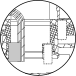
\includepdf[landscape=true]{img/DR2.pdf}


\clearpage

\ifdef{\public}{\end{document}}{}

\newpage

\pagestyle{correction}

\section{Correction}

\subsection{Conception d'un corps support}

\begin{center}
\includegraphics[width=\textwidth]{img/Support_cor.pdf}
\end{center}

\subsection{Conception d'un corps d’affûteuse}

\begin{center}
\includegraphics[width=\textwidth]{img/Corps_affuteuse_prive}
\end{center}

\section{Système d'enfouissement de câbles sous-marins}

\paragraph{Question 1:}

\begin{center}
\includegraphics[width=\textwidth]{img/dessin_palier}
\end{center}

\paragraph{Question 2:}

\begin{enumerate}
 \item Pliage de la tôle en U.
 \item Soudage des deux plaques intérieures latérales,
 \item Soudage de la plaque intérieure de face,
 \item Perçage des 4 trous.
\end{enumerate}

\end{document}
